\section{总结与展望}
\miniframesoff
  \frame
  {
    \frametitle{\secname~ }
    \footnotesize
    \begin{block}{总结}
    \begin{itemize}
        \item 提出了确定性增量梯度方法SIG和SIG-M
        \item 证明了SIG达到线性收敛,并将其推广到单调算子的零点问题
        \item 实验结果表明,SIG在大规模优化问题上对内存友好,优于现有的算法;
              动量的引入对SIG算法起到了加速的作用
    \end{itemize}
    \end{block}

    \pause

    \begin{block}{未来工作}
    \begin{itemize}
        \item 改进SIG的理论收敛率
        \item SIG-M的收敛性分析
        \item 将SIG推广到更一般的带非光滑正则项的优化问题
        \item 设计和分析异步或分布式的变种算法
    \end{itemize}
    \end{block}
  }

  \frame
  {
    \frametitle{致谢}
    \footnotesize

    % \begin{overlayarea}{11.5cm}{8cm}
    % {
    %     \only<1-2>
    %     {
    %         \begin{itemize}
    %             \item 感谢钱徽教授对本文选题和写作的指导
    %             \item 感谢沈泽邦学长、张超学长、周腾飞学长对本文提出的宝贵意见以及在凸优化理论方面对我的指导
    %             \item 感谢我的家人对我学业的支持
    %             \item 感谢学校和学院的培养
    %         \end{itemize}
    %         \pause
    %         本工作已被第21届人工智能与统计会议(AISTATS 2018)录用及发表: \\
    %         Jiahao Xie, Hui Qian, Zebang Shen and Chao Zhang. Towards Memory-Friendly Deterministic Incremental Gradient Method. AISTATS 2018.
    %         \begin{figure}[H]
    %             
\includegraphics{data/img/logo}
    %         \end{figure}
    %     }
    %     \only<3>
    %     {
    %         \begin{figure}[H]
    %             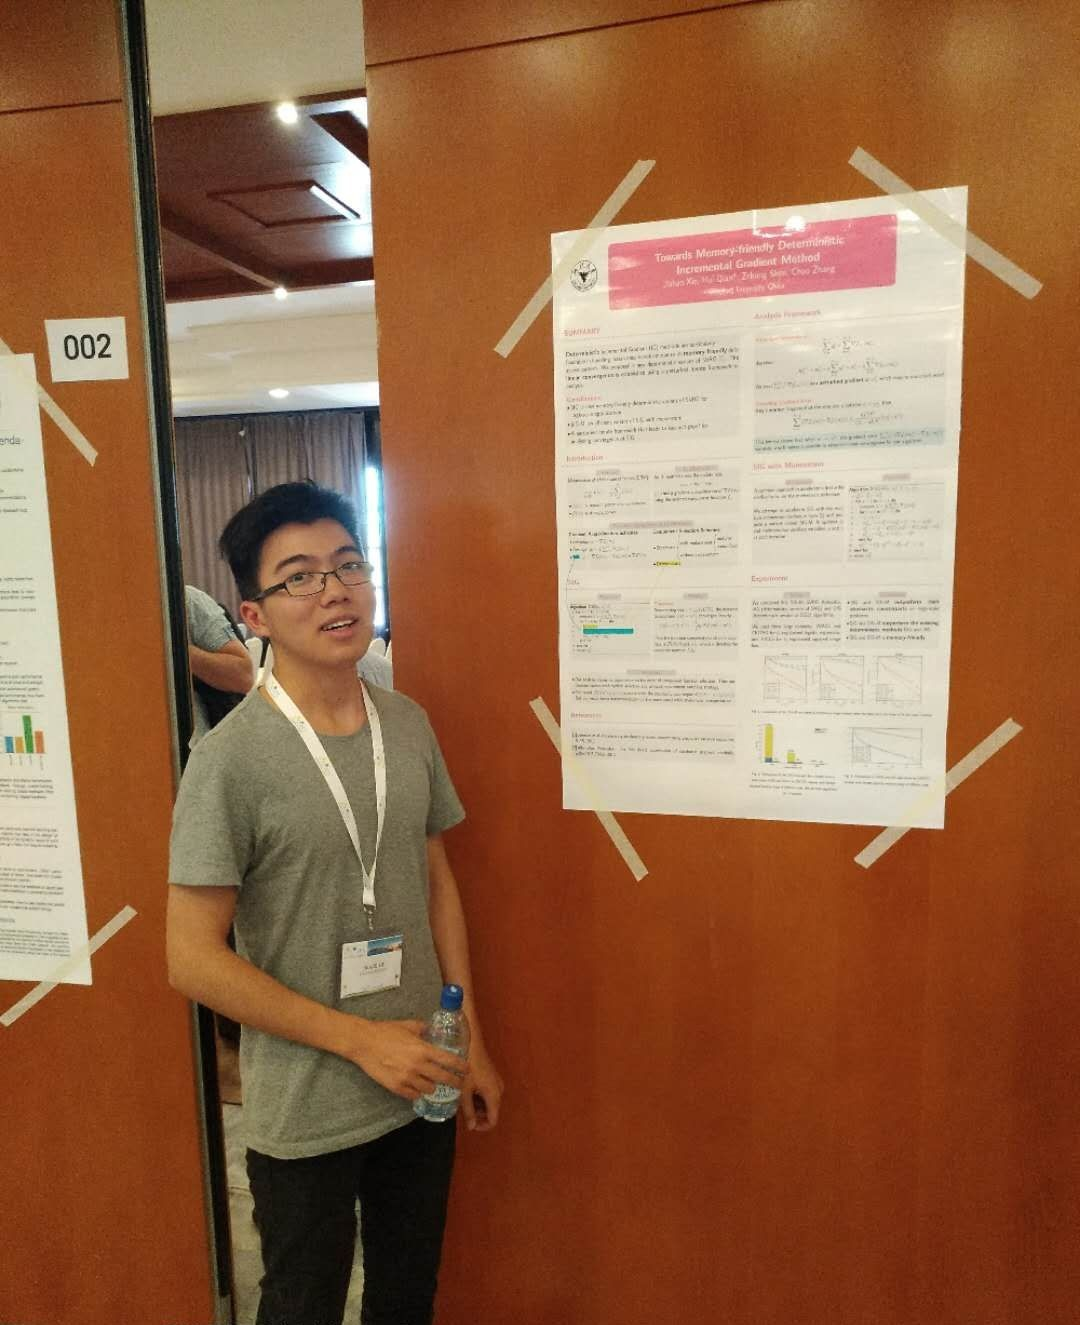
\includegraphics[trim={0 0 0 0},clip,height=8cm]{data/img/jiahao_xie}
    %         \end{figure}
    %     }
    % }
    % \end{overlayarea}

    \begin{itemize}
        \item 感谢钱徽教授对本文选题和写作的指导
        \item 感谢沈泽邦学长、张超学长、周腾飞学长对本文提出的宝贵意见以及在凸优化理论方面对我的指导
        \item 感谢我的家人对我学业的支持
        \item 感谢学校和学院的培养
    \end{itemize}
    % \pause
    % 本工作已被第21届人工智能与统计会议(AISTATS 2018)录用及发表: \\
    % Jiahao Xie, Hui Qian, Zebang Shen and Chao Zhang. Towards Memory-Friendly Deterministic Incremental Gradient Method. AISTATS 2018.
    % \begin{figure}[H]
    %     
\includegraphics{data/img/logo}
    % \end{figure}
    % \begin{figure}[H]
    %     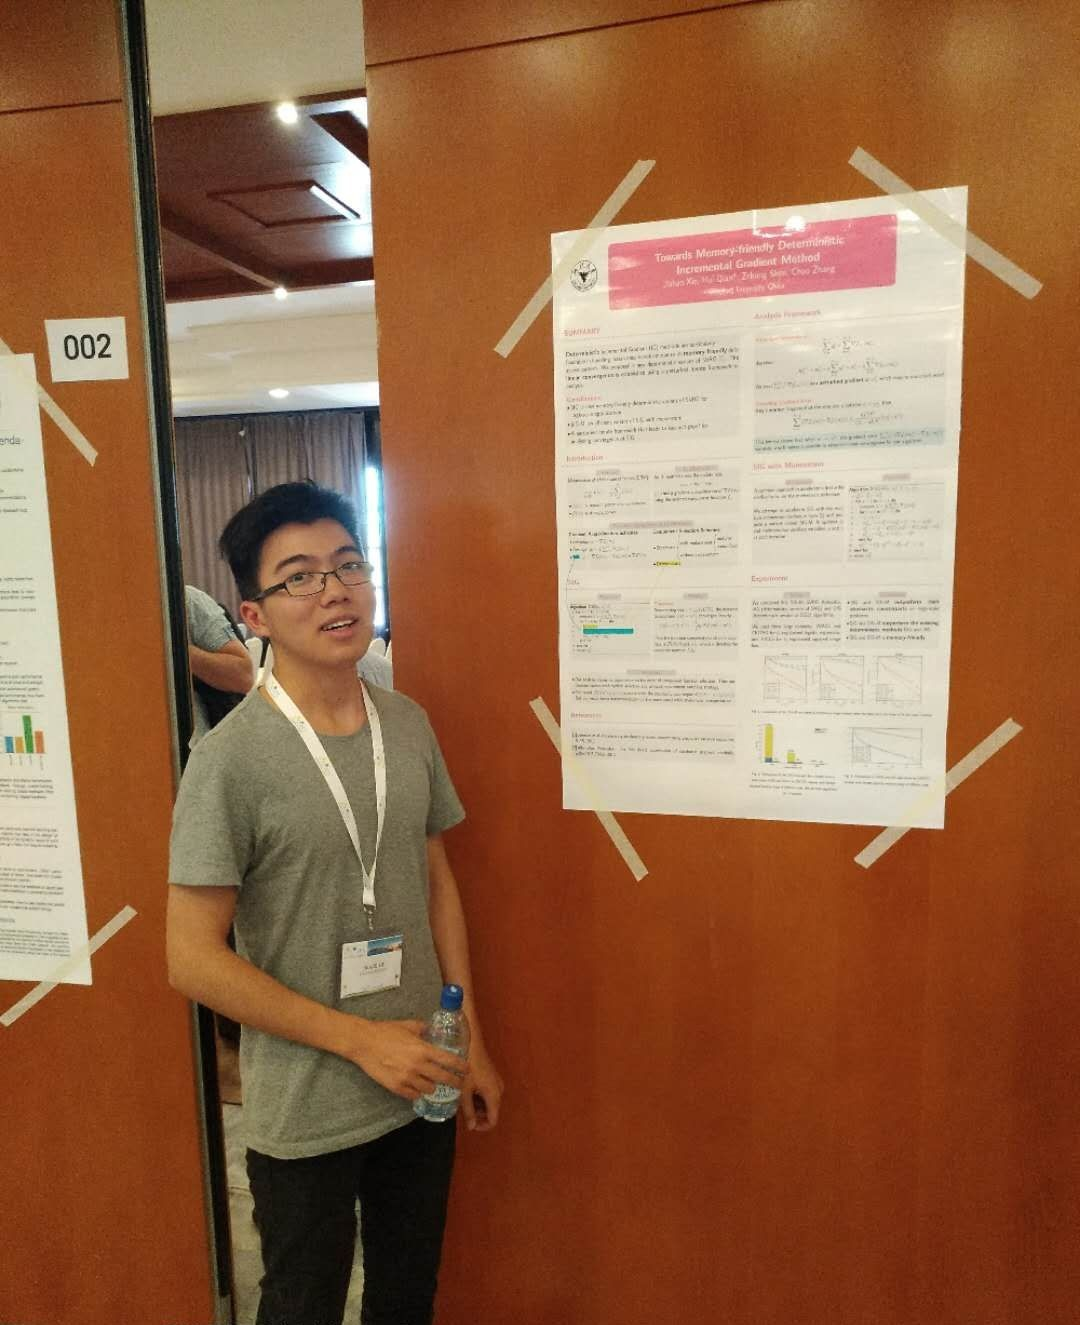
\includegraphics[trim={0 0 0 0},clip,height=8cm]{data/img/jiahao_xie}
    % \end{figure}
  }

  \frame
  {
    \frametitle{Q \& A}
    \begin{block}{Questions?}
      ~\\ ~\\
      \center{\Large{Thank you!}}
      \\ ~\\ ~\\ ~\\ ~\\
    \end{block}
  }
